\documentclass[pdfa,cucitura]{toptesi}
\hypersetup{%
	pdfpagemode={UseOutlines},
	bookmarksopen,
	pdfstartview={FitH},
	colorlinks,
	linkcolor={blue},
	citecolor={red},
	urlcolor={blue}
}

\usepackage[latin1]{inputenc}

% exact placing figures
\usepackage{float}

% insert eps files
\usepackage{epstopdf}

% cool tables
\usepackage{booktabs}
\usepackage{rotating}

\usepackage{mathrsfs}
\usepackage{amsmath}

\selectlanguage{english}

\ateneo{Politecnico di Torino}
\titolo{Building Trustworthiness Into Marketplaces}

\corsodilaurea{Computer Engineering}

\candidato{Marco \textsc{Terrinoni}}
\relatore{prof.\ Antonio Lioy}
%\tutoreaziendale{Stuart Short}

\sedutadilaurea{\textsc{Anno~accademico} 2013-2014}
\logosede{img/logopolito}

% per inserire uno spazio "fantasma" nella definizione di un'abbreviazione
\usepackage{xspace}

% per inserire un DOI senza problemi coi caratteri "strani" ivi presenti
\usepackage{doi}
\renewcommand{\doitext}{DOI }% originally was "doi:"

% per inserire correttamente le unit� di misura SI (incluse quelle binarie)
\usepackage[binary-units]{siunitx}
% se si desidera usare / invece che la potenza -1 per indicare "al secondo"
\sisetup{per-mode=symbol}

% per inserire codice di programmazione complesso
\usepackage{listings}% per inserire codice di programmazione complesso
\lstset{
basicstyle=\ttfamily,
columns=fullflexible,
xleftmargin=3ex,
breaklines,
breakatwhitespace,
escapechar=`
}

% modify some page parameters
\setlength{\parskip}{\medskipamount}
\advance\voffset -5mm
\advance\textheight 30mm

% riga orizzontale
\newcommand{\HRule}{\rule{\linewidth}{0.2mm}}
% esempio di creazione di semplici abbreviazioni
\newcommand{\ltx}{\LaTeX\xspace}
\newcommand{\txw}{TeXworks\xspace}
\newcommand{\mik}{MikTex\xspace}
\newcommand{\html}{HTML\xspace}
\newcommand{\xhtml}{XHTML\xspace}
\newcommand*\rot{\rotatebox{90}}

\newcommand{\latex}{\LaTeX\xspace}

% esempio di creazione di un'abbreviazione con un parametro (il cui uso � indicato da #1)
\newcommand{\cmd}[1]{\texttt{#1}\xspace}
% per citare un RFC, es. \rfc{822}
\newcommand{\rfc}[1]{RFC-#1\xspace}
% per citare un file (es. \file{autoexec.bat}) o una URI fittizia (es. \file{http://www.lioy.it/})
% per le URI vere usare \url o \href
\newcommand{\file}[1]{\texttt{#1}\xspace}
% per inserire codice di esempio in-line
\newcommand{\code}[1]{\lstinline|#1|}
% importante per i pathname Windows perch� non si pu� usare \ essendo un carattere riservato di Latex
\newcommand{\bs}{\textbackslash}
% definizione di un termine: formattazione ed inserimento nell'indice
\newcommand{\tdef}[1]{\textit{#1}\index{#1}}
% meta-termine, usato tipicamente nelle definizioni dei tag
\newcommand{\meta}[1]{\textit{#1}}

\begin{document}
\english

\errorcontextlines=9

\expandafter\ifx\csname StileTrieste\endcsname\relax
%\frontespizio
\else
	\paginavuota
	\begin{dedica}
		To my grandparents

		\textdagger\ You will always live in my memories
	\end{dedica}
	\tomo
\fi

\sommario
This document collects the various personal notes from the course ``Formal Languages and Compilers'' (2012), prof. Silvano Rivoira.
The \latex source code is available in a dedicated \href{https://github.com/terrinoni/FormalLanguagesAndCompilers-Notes}{GitHub repository}.

\indici

\mainmatter

\part{Formal Languages}

\chapter{Classification (FLC)}
\section{Grammars}
A grammar is a 4-tuple $G = (N, T, P, S)$ where:
\begin{description}
	\item[$N:$] alphabet of \underline{non-terminal} symbols;
	\item[$T:$] alphabet of \underline{terminal} symbols:
	\begin{itemize}
		\item $N \cap T = 0$ (two alphabets are disjoined),
		\item $V = N \cup T$ (alphabet of the grammar);
	\end{itemize}
	\item[$P:$] finite set of rules (productions);
	\item[$S:$] start (non-terminal) symbol.
\end{description}

A language produced by $G = (N, T, P, S)$ is:
$$
	L(G) = \left\{w \middle| w \in T^\ast; S \Rightarrow^\ast w\right\}
$$
Grammars that produce the same languages are said ``equivalent''.

\subsection{Types of Grammars}
\begin{description}
	\item[Type 0 grammars] (phase-structure)
		$$
			P = \left\{\alpha \to \beta \middle| \alpha \in V^+; \alpha \notin T^+; \beta \in V^\ast \right\}
		$$
	\item[Type 1 grammars] (context-sensitive)
		$$
			P = \left\{\alpha \to \beta \middle| \alpha \in V^+; \alpha \notin T^+; \beta \in V^+; |\alpha| \leq |\beta| \right\}
		$$
	\item[Type 2 grammars] (context-free)
		$$
			P = \left\{A \to \beta \middle| A \in N; \beta \in V^+ \right\}
		$$
\end{description}

\subsection{Linear Grammars}
$$
	P = \left\{A \to xBy, A \to x \middle| A, B \in N; x,y \in T^+ \right\}
$$
\begin{description}
	\item[Type 3 grammars] (right/left - linear)
	\begin{itemize}
		\item Right-Linear grammars
			$$
				P = \left\{A \to xB, A \to x \middle| A, B \in N; x \in T^+ \right\}
			$$
		\item Left-Linear grammars
			$$
				P = \left\{A \to Bx, A \to x \middle| A, B \in N; x \in T^+ \right\}
			$$
	\end{itemize}
	\item[Type 3 grammars] (right/left - regular)
	\begin{itemize}
		\item Right-Regular grammars
			$$
				P = \left\{A \to aB, A \to a \middle| A, B \in N; a \in T \right\}
			$$
		\item Left-Regular grammars
			$$
				P = \left\{A \to Ba, A \to a \middle| A, B \in N; a \in T \right\}
			$$
	\end{itemize}
\end{description}

\chapter{Regular Languages (RL)}
\section{Deterministic Finite Automata (DFA)}
A DFA is a 5-tuple $A = (Q, \Sigma, \delta, q_0, F)$ where:
\begin{description}
	\item[$Q:$] finite (non-empty) set of states;
	\item[$\Sigma:$] alphabet of input symbols;
	\item[$\delta:$] transition function:
		$$
			\delta: Q \times \Sigma \to Q
		$$
	\item[$q_0:$] start state:
		$$
			q_0 \in Q
		$$
	\item[$F:$] set of final states:
		$$
			F \subseteq Q
		$$
\end{description}

\subsection{Transition Table}
Transitional Table is a tabular representation of this transition function.

\subsection{Transition Diagram}
Transitional Diagram is a graph where:
\begin{itemize}
	\item for each state in the automaton there a node;
	\item for each transition $\delta(p, a) = q$ there is an arc from $p$ to $q$ labelled $a$.
\end{itemize}
The start state has an entering non-labelled arc and the final states are marked by a double circle.

\section{Non-Deterministic Finite Automata (NFA)}
An NFA is a 5-tuple $A = (Q, \Sigma, \delta, q_0, F)$ where:
\begin{description}
	\item[$Q:$] finite (non-empty) set of states;
	\item[$\Sigma:$] alphabet of input symbols;
	\item[$\delta:$] transition function:
		$$
			\delta: Q \times \Sigma \to \mathscr{P}(Q)
		$$
		$\mathscr{P}(Q)$: powerset of Q (the set of all subsets)
		$$
			\|\mathscr{P}(Q)\| = 2^{\|Q\|}
		$$
	\item[$q_0:$] start state:
		$$
			q_0 \in Q
		$$
	\item[$F:$] set of final states:
		$$
			F \subseteq Q
		$$
\end{description}
NB: a DFA is a special case of NFA.

\section{Equivalence of NFA and DFA}
\begin{figure}[H]
    \centerline{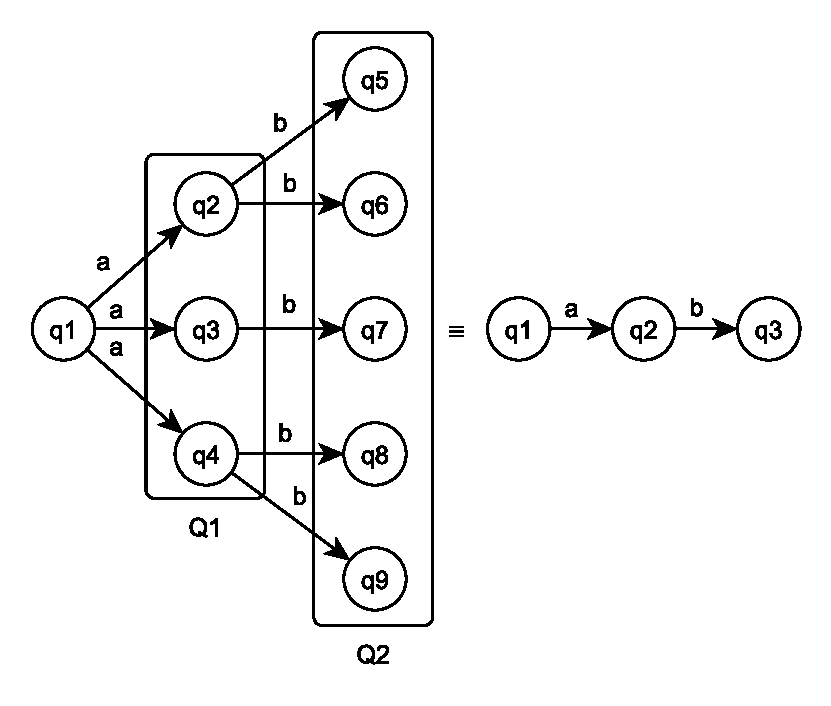
\includegraphics[width=0.6\textwidth]{img/1.pdf}}
\end{figure}
\begin{align*}
	Q_1 &= \left\{q_2, q_3, q_4\right\}\\
	Q_2 &= \left\{q_5, q_6, q_7, q_8, q_9\right\}
\end{align*}

Let $N = (Q_n, \Sigma, \delta_n, q_0, F_n)$ be an NFA; let us construct a DFA $D = (Q_d, \Sigma, \delta_d, \left\{q_0\right\}, F_d)$ where:
\begin{itemize}
	\item $Q_d \subseteq \mathscr{P}(Q_n)$;
	\item $\delta_d(S, a) = \cup_i \delta_n(p_1, a)$ where $p_i \in S \in Q_d$;
	\item $F_d = \left\{S \middle| S \in Q_d; S \cap F_n \neq \emptyset \right\}$.
\end{itemize}
By construction $L(D) = L(N)$, so $NFA \equiv DFA$

\section{From Finite Automata to Regular Expression}
It is possible to eliminate states in a Finite Automata by maintaining all the paths and by labelling the transitions with regular expressions:
\begin{figure}[H]
	\centerline{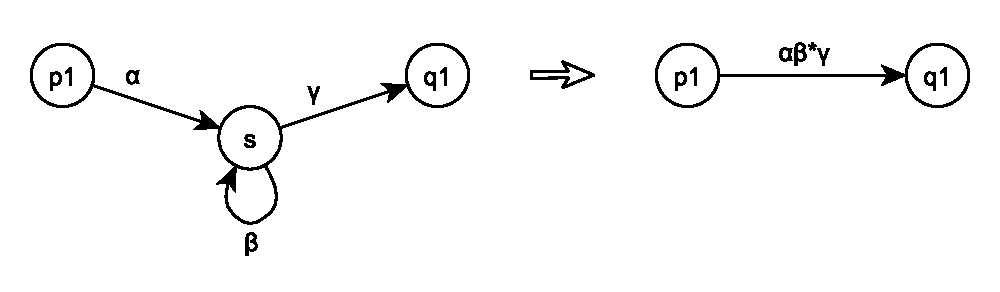
\includegraphics[width=0.7\textwidth]{img/2.pdf}}
\end{figure}
Given a finite state automaton $FA = (Q, \Sigma, \delta, q_0, F)$, add an initial state $A$ and a final state $\Omega$:
\begin{figure}[H]
	\centerline{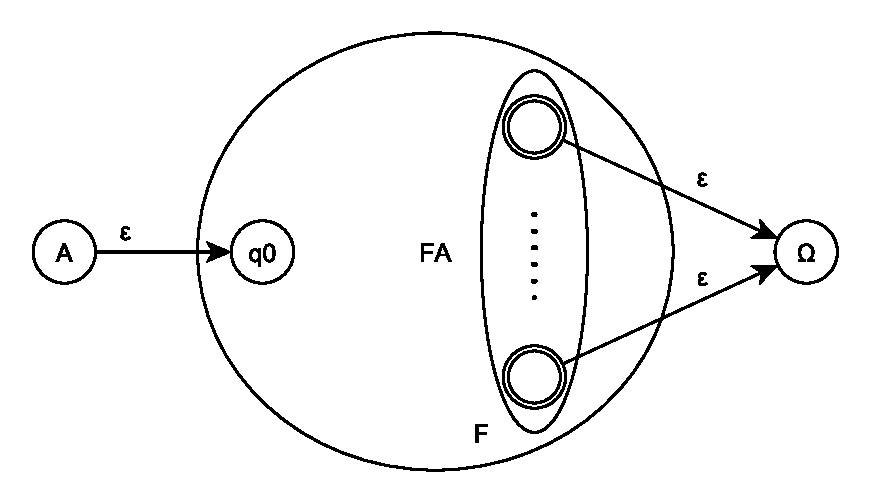
\includegraphics[width=0.7\textwidth]{img/3.pdf}}
\end{figure}
\begin{itemize}
	\item eliminate all the states in $FA$;
	\item the union of the labels on the transitions from $A$ to $\Omega$ gives the regular expression of the language $L(FA)$.
\end{itemize}

\section{From Regular Expression to Finite Automata}

\subsection{Regular Sets}
The regular sets: $0$, $\left\{\varepsilon\right\}$, $\left\{a\right\}$, $a \in \Sigma$ are accepted by finite state automata.
\begin{figure}[H]
	\centerline{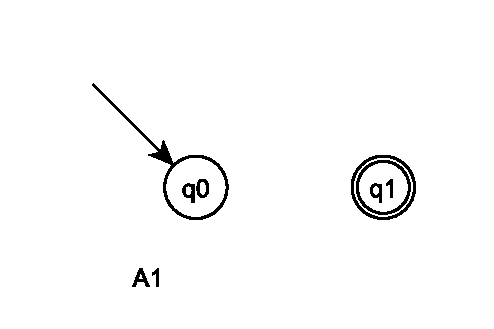
\includegraphics[width=0.4\textwidth]{img/4.pdf}}
\end{figure}
$$
	L(A_1) = 0
$$
\begin{figure}[H]
	\centerline{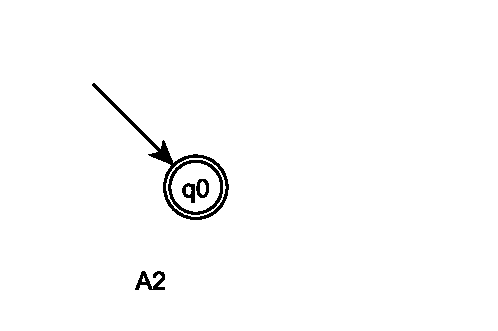
\includegraphics[width=0.4\textwidth]{img/5.pdf}}
\end{figure}
$$
	L(A_2) = \left\{\varepsilon\right\}
$$
\begin{figure}[H]
	\centerline{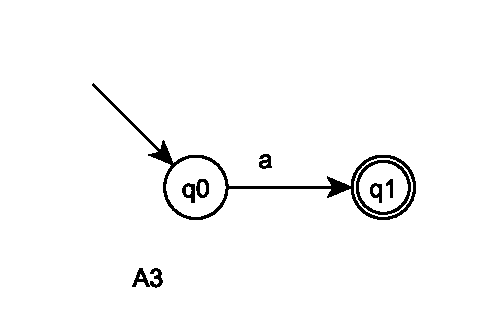
\includegraphics[width=0.4\textwidth]{img/6.pdf}}
\end{figure}
$$
	L(A_3) = \left\{a\right\}, a \in \Sigma
$$
Let $A_1 = (Q_1, \Sigma, \delta_1, q_{01}, F_1)$ and $A = (Q_2, \Sigma, \delta_2, q_{02}, F_2)$ be finite state automata; the language $L(A_1) \cup L(A_2)$ is accepted by a finite state automaton $A_4$:
\begin{figure}[H]
	\centerline{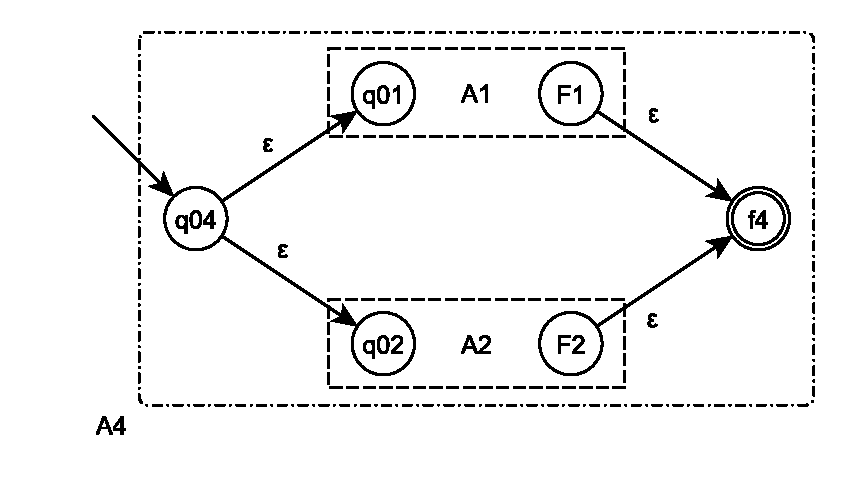
\includegraphics[width=0.7\textwidth]{img/7.pdf}}
\end{figure}

The language $L(A_1)L(A_2)$ is accepted by a finite state automaton $A_5$:
\begin{figure}[H]
	\centerline{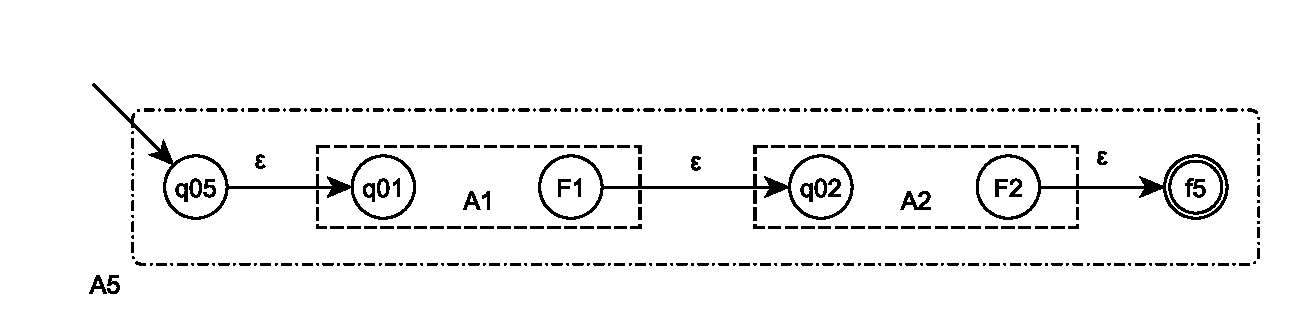
\includegraphics[width=1\textwidth]{img/8.pdf}}
\end{figure}

The language $L(A_1)^\ast$ is accepted by a finite state automaton $A_6$:
\begin{figure}[H]
	\centerline{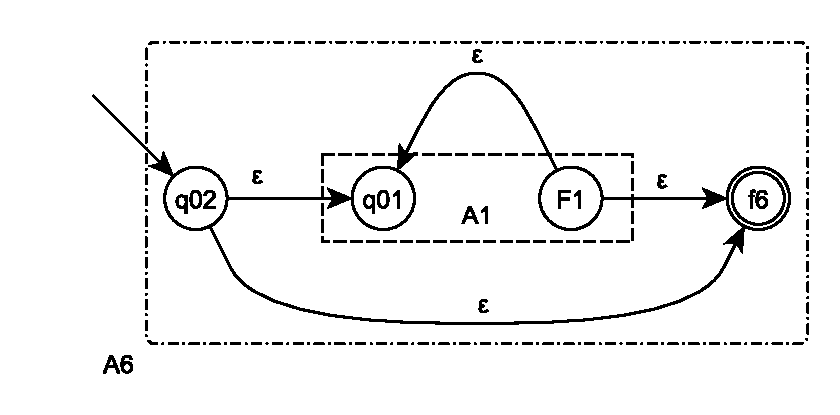
\includegraphics[width=0.7\textwidth]{img/9.pdf}}
\end{figure}

\section{Non-Deterministic Finite State Automata with $\varepsilon\text{-transition}$ ($\varepsilon\text{-NFA}$)}
In the construction of a Finite State Automaton from regular expressions, the $\varepsilon\text{-transitions}$ make the automata \emph{non-deterministic}.
The function $\varepsilon\text{-closure}(q)$ gives the set of states that can be reached (recursively) from state $q$ with empty string.

\subsection{Equivalence of $\varepsilon\text{-NFA}$ and DFA}
Let $N = (Q_n, \Sigma, \delta_n, q_0, F_n)$ be an $\varepsilon\text{-NFA}$; let us construct a DFA $D = (Q_d, \Sigma, \delta_d, \varepsilon\text{-closure}(q_0), F_d)$ where:
\begin{itemize}
	\item $Q_d \subseteq \mathscr{P}(Q_n)$;
	\item $\delta_d(S, a) = \varepsilon\text{-closure}(\cup_i \delta_n(p_i, a))$ where $p_i \in S \in Q_d$;
	\item $F_d \left\{S \middle| S \in Q_d; S \cap F_n \neq \emptyset\right\}$
\end{itemize}
By construction $L(D) = L(N)$.

\section{Finite Automaton $\equiv$ Regular Languages}
\begin{itemize}
	\item Let $G = (N, T, P, S)$ be a \underline{Right-Regular} grammar; let us construct an FA $A = (Q, T, \delta, S, F)$ where:
	\begin{itemize}
		\item $Q = N \cup \left\{\Omega\right\}$ with $\Omega \in N$;
		\item $F = \left\{\Omega\right\}$;
		\item $
			\delta = \begin{Bmatrix}
				\delta(A, a) = B \quad \text{if} \quad A \to aB \in P \\
				\delta(A, a) = \Omega \quad \text{if} \quad A \to a \in P
			\end{Bmatrix}
		$
	\end{itemize}
	By construction $L(G) = L(A)$.
	\item Let $G = (N, T, P, S)$ be a \underline{Left-Regular} grammar; let us construct an FA $A = (Q, T, \delta, I, \left\{S\right\})$ where:
	\begin{itemize}
		\item $Q = N \cup \left\{I\right\} \quad \text{with} \quad I \notin N$;
		\item $F = \left\{S\right\}$;
		\item $
			\delta = \begin{Bmatrix}
				\delta(B, a) = B \quad \text{if} \quad A \to Ba \in P \\
				\delta(I, a) = \Omega \quad \text{if} \quad A \to a \in P
			\end{Bmatrix}
		$
	\end{itemize}
	By construction $L(G) = L(A)$.
\end{itemize}

\section{Minimum-State DFA}
Let $DFA = (Q, \Sigma, \delta, q_0, F)$ be a deterministic finite automaton, then:
\begin{itemize}
	\item two states $p$ and $q$ of DFA are distinguishable if there is a string $w \in \Sigma^\ast$ such that $\delta(p, w) \in F$ and $\delta(q, w) \in F$;
	\item two states $p$ and $q$ of DFA are equivalent ($p \equiv q$) if they are \emph{non-distinguishable} for any string $w \in \Sigma^\ast$.
\end{itemize}
A DFA is \emph{minimum-state} if it does not contain equivalent states.

Two states $p$ and $q$ of a DFA are $m\text{-equivalent}$ ($p \equiv_m q$) if they are non-distinguishable for all strings $w \in \Sigma^\ast$ with $\|w\| \leq m$.
The equivalent states can be determined by partitioning the set $Q$ in classes of $m\text{-equivalent}$ states, for $m = 0, 1, \ldots, \|Q\| - 2$.

\section{Complement of a Regular Language}
The complement of a regular language is a regular language.

Let $DFA = (Q, \Sigma, \delta, q_0, F)$ be a completely specified deterministic finite automaton, that is there is a transition on every symbol of $\Sigma$ from every state.
The automaton $DFA_c = (Q, \Sigma, q_0, Q - F)$ accepts the language
$$
	L(DFA_c) = \Sigma^\ast - L(DFA) = \neg L(DFA)
$$

\section{Intersection of Regular Languages}
The intersection of two regular languages is a regular language.
$$
	L_1 \cap L_2 = \neg (\neg L_1 \cup \neg L_2)
$$
Let $DFA_1 = (Q_1, \Sigma, \delta_1, q_{01}, F_1)$ and $DFA_2 = (Q_2, \Sigma, \delta_2, q_{02}, F_2)$; the automaton $DFA1 = (Q_1 \times Q_2, \Sigma, \delta, (q_{01}, q_{02}), F_1 \times F_2)$ accepts the language
$$
	L(DFA_1) = L(DFA1) \cap L(DFA_2)
$$

\section{Equivalence of Regular Languages}
It is possible to test if two regular languages are the same:
\begin{itemize}
	\item $DFA_1 = (Q_1, \Sigma, \delta_1, q_{01}, F_1)$;
	\item $DFA_2 = (Q_2, \Sigma, \delta_2, q_{02}, F_2)$.
\end{itemize}
Let us find the equivalence states in the set $Q_1 \cup Q_2$:
$$
	\text{if} \quad q_{01} \equiv q_{02} \quad \text{then} \quad L(DFA_1) = L(DFA_2)
$$

\chapter{Context-Free Languages (CFL)}
\section{Parse Trees}
A parse tree for a context-free grammar (CFG) $G = (N, T, P, S)$ is a tree where:
\begin{itemize}
    \item the root is labelled by the start symbol;
    \item each interior node is labelled by a symbol in $N$;
    \item each leaf is labelled by a symbol in $N \cup T \cup \left\{\varepsilon\right\}$;
    \item an interior node labelled by $A$ has a children labelled by $x_1, x_2, \ldots, x_n$ only if $A \to x_1, x_2, \ldots, x_n$ is a production of $P$.
\end{itemize}
Yield of a parse tree is a string obtained by concatenating the labels of the leaves.

\section{Leftmost/Rightmost Derivation}
\subsubsection{Leftmost Derivation}
The leftmost non-terminal symbol is replaced at each derivation step.
\subsubsection{Rightmost Derivation}
The rightmost non-terminal symbol is replaced at each derivation step.

\section{Ambiguity}
Every string in a CFL has at least one parse tree; each parse tree has just one leftmost derivation and just one rightmost derivation.
A context-free grammar is \emph{ambiguous} if there is at least one string in its language having two different parse trees; a CFL is inherently ambiguous if all its grammars are ambiguous.

\section{Eliminating Useless Symbols in a Context-Free Grammar}
A symbol $X$ is useful for a $CFG = (N, T, P, S)$ if there is some derivations $S \Rightarrow^\ast aX\beta \Rightarrow^\ast w \in T^\ast$.
\begin{itemize}
    \item a useful symbol $X$ generates a non-empty languages: $X \Rightarrow^\ast x \in T^\ast$;
    \item a useful symbol $X$ is reachable: $S \Rightarrow^\ast \alpha X\beta$.
\end{itemize}
Eliminating useless symbols from a grammar will not change the generated language:
\begin{enumerate}
    \item eliminate symbols generating an empty language;
    \item eliminate unreachable symbols.
\end{enumerate}
\subsubsection{Finding Symbols Generating Non-Empty Languages}
\begin{itemize}
    \item every symbol of $T$ generates a non-empty language;
    \item if $A \to \alpha$ and all symbols in $\alpha$ generate a non-empty language, then $A$ generates a non-empty language.
\end{itemize}
\subsubsection{Finding Reachable Symbols}
\begin{itemize}
    \item the start symbol $S$ is reachable;
    \item if $A \to \alpha$ and $A$ is reachable, all symbols in $\alpha$ are reachable.
\end{itemize}

\section{$\varepsilon\text{-productions}$ in CFG}
According to the Chomsky classification, only \emph{Type 0 grammars} can have $\varepsilon\text{-productions}$; anyway the languages generated by CFGs that contain $\varepsilon\text{-productions}$ are CFL.

A context-free grammar $G_1$ with $\varepsilon\text{-productions}$ can be transformed into an equivalent CFG $G_2$ without $\varepsilon\text{-productions}$:
$$
    L(G_2) = L(G_1) - \left\{\varepsilon\right\}
$$
If $A \to x_1, \ldots, x_i, \ldots, x_n$ is in $P_1$ and $x_i \Rightarrow^\ast \varepsilon$, then $P_2$ will contain $A \to x_1 \ldots x_i \ldots x_n$ and $A \to x_1 \ldots x_{i - 1} x_{i + 1} \ldots x_n$.

\section{Pushdown Automata (PDA)}
A PDA is a 7-tuple $P = (Q, \Sigma, \Gamma, \delta, q_0, Z_0, F)$ where:
\begin{description}
    \item[$Q:$] finite (non-empty) set of states;
    \item[$\Sigma:$] alphabet of input symbols;
    \item[$\Gamma:$] alphabet of stack symbols;
    \item[$\delta:$] transition function
    $$
        \delta: Q \times (\Sigma \cup \left\{\varepsilon\right\}) \times \Gamma \to \left\{(p, \gamma) \middle| p \in Q; \gamma \in \Gamma^\ast \right\}
    $$
    \item[$q_0:$] start state ($q_0 \in Q$);
    \item[$Z_0:$] start stack symbol ($Z_0 \in \Gamma$);
    \item[$F:$] set of final states ($F \subseteq Q$).
\end{description}

\subsection{Transitions of a PDA}
\begin{itemize}
    \item $\delta(q,a,x) = \left\{(p_1, \gamma_1), \ldots, (p_m, \gamma_m)\right\}$
    From state $q$, with $a$ in input and $x$ on top of the stack:
    \begin{enumerate}
        \item consumes $a$ from the input string;
        \item goes to a state $p_i$ and replace $x$ with $\gamma_i$ (the first symbol of $\gamma_i$ goes on top of the stack).
    \end{enumerate}
    \item $\delta(q,\varepsilon,x) = \left\{(p_1, \gamma_1), \ldots, (p_m, \gamma_m)\right\}$
    From state $q$, with $x$ on top of the stack:
    \begin{enumerate}
        \item no input symbol is consumed;
        \item goes to a state $p_i$ and replaces $x$ with $\gamma_i$ (the first symbol of the stack).
    \end{enumerate}
\end{itemize}

\subsection{Languages Accepted by a PDA}
Language accepted by final state by PDA:
$$
    P = (Q, \Sigma, \Gamma, \delta, q_0, Z_0, F)
$$
$$
    L(P) = \left\{w \middle| w \in \Sigma^\ast; (q_0, w, Z_0) \to^\ast (q, \varepsilon, \alpha); q \in F \right\}
$$
Language accepted by empty stack by the PDA:
$$
    P = (Q, \Sigma, \Gamma, \delta, q_0, Z_0, \emptyset)
$$
$$
    N(P) = \left\{w \middle| w \in \Sigma^\ast; (q_0, w, Z_0) \to^\ast (q, \varepsilon, \varepsilon) \right\}
$$

\subsection{PDA Languages $\equiv$ Context-Free Languages}
Let $G = (N, T, P, S)$ be a context-free grammar; let us construct a $PDA = (\left\{q\right\}, T, \Gamma, \delta, q, S, \emptyset)$ where:
\begin{itemize}
    \item $\Gamma = N \cup T$;
    \item $\delta = \begin{Bmatrix}
        \delta(q, \varepsilon, A) = \left\{(q, \alpha) \quad \text{for each} \quad A \to \alpha \in P \right\} \\
        \delta(q, a, a) = \left\{(q, \varepsilon) \quad \text{for each} \quad a \in T \right\}
        \end{Bmatrix}$
\end{itemize}
PDA accepts $L(G)$ by empty stack, making a sequence of transitions corresponding to a leftmost derivation.

\chapter{Turing Machines (TM)}

\part{Compilers}

\chapter{Compiler Structure (CS)}
\section{Compiler Structure}
\begin{figure}[H]
    \centerline{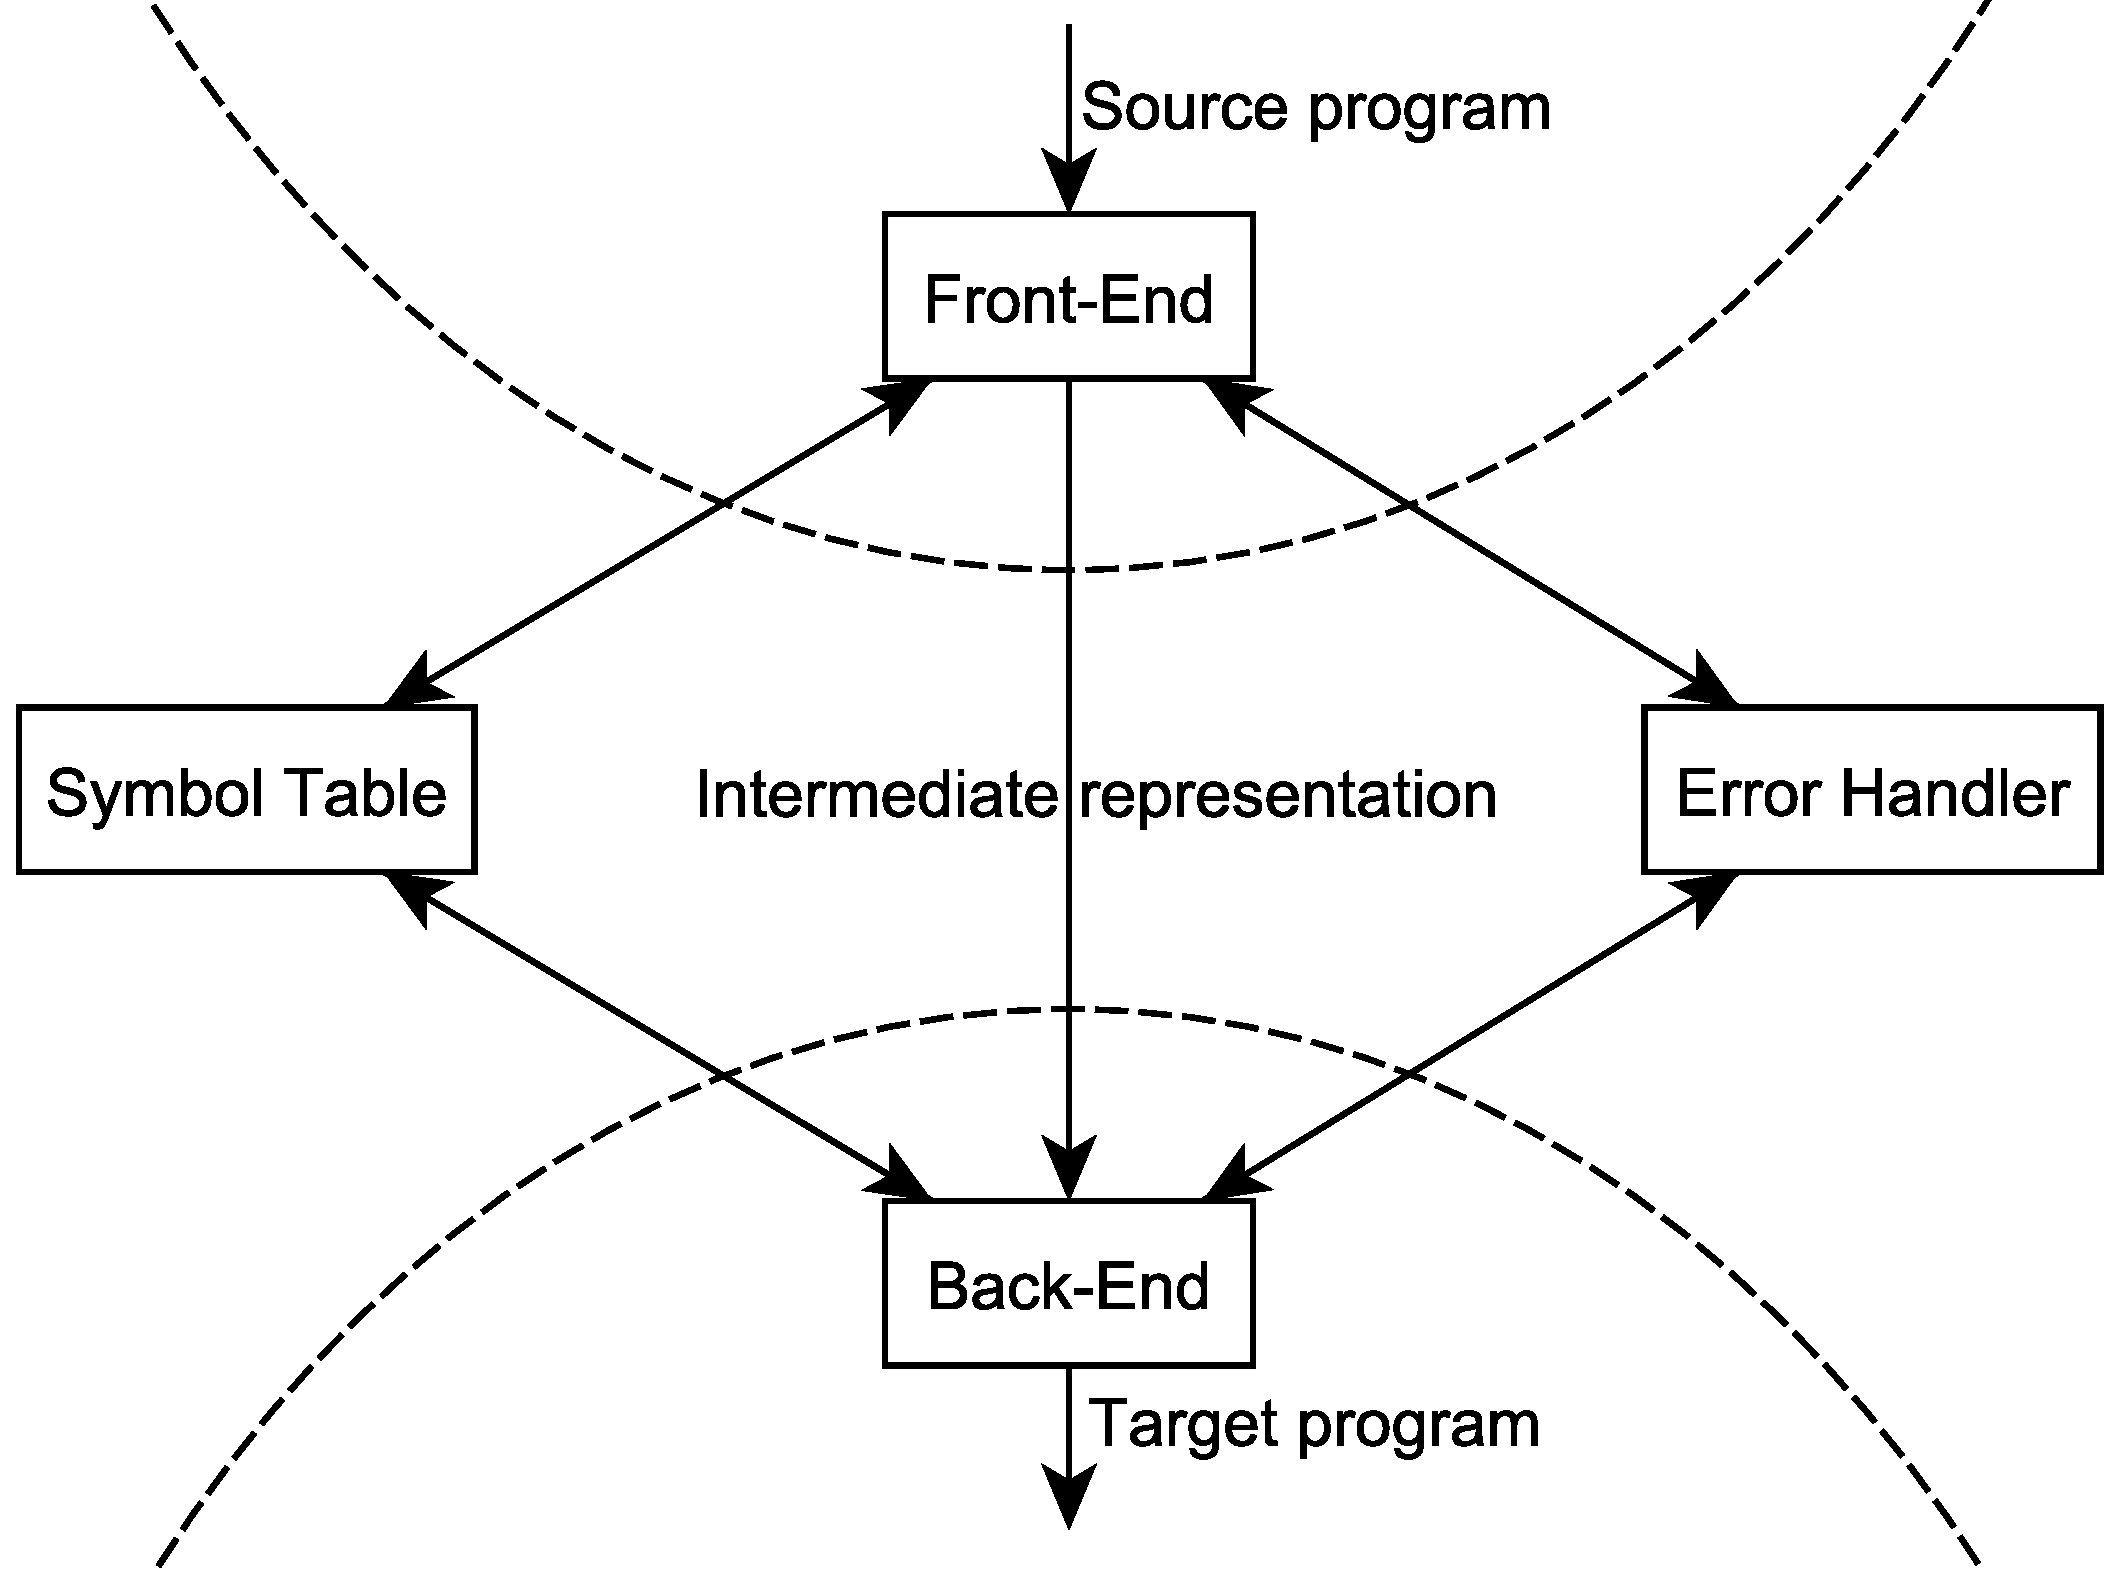
\includegraphics[width=0.7\textwidth]{img/10.pdf}}
\end{figure}

\subsection{Front-End}
\begin{figure}[H]
    \centerline{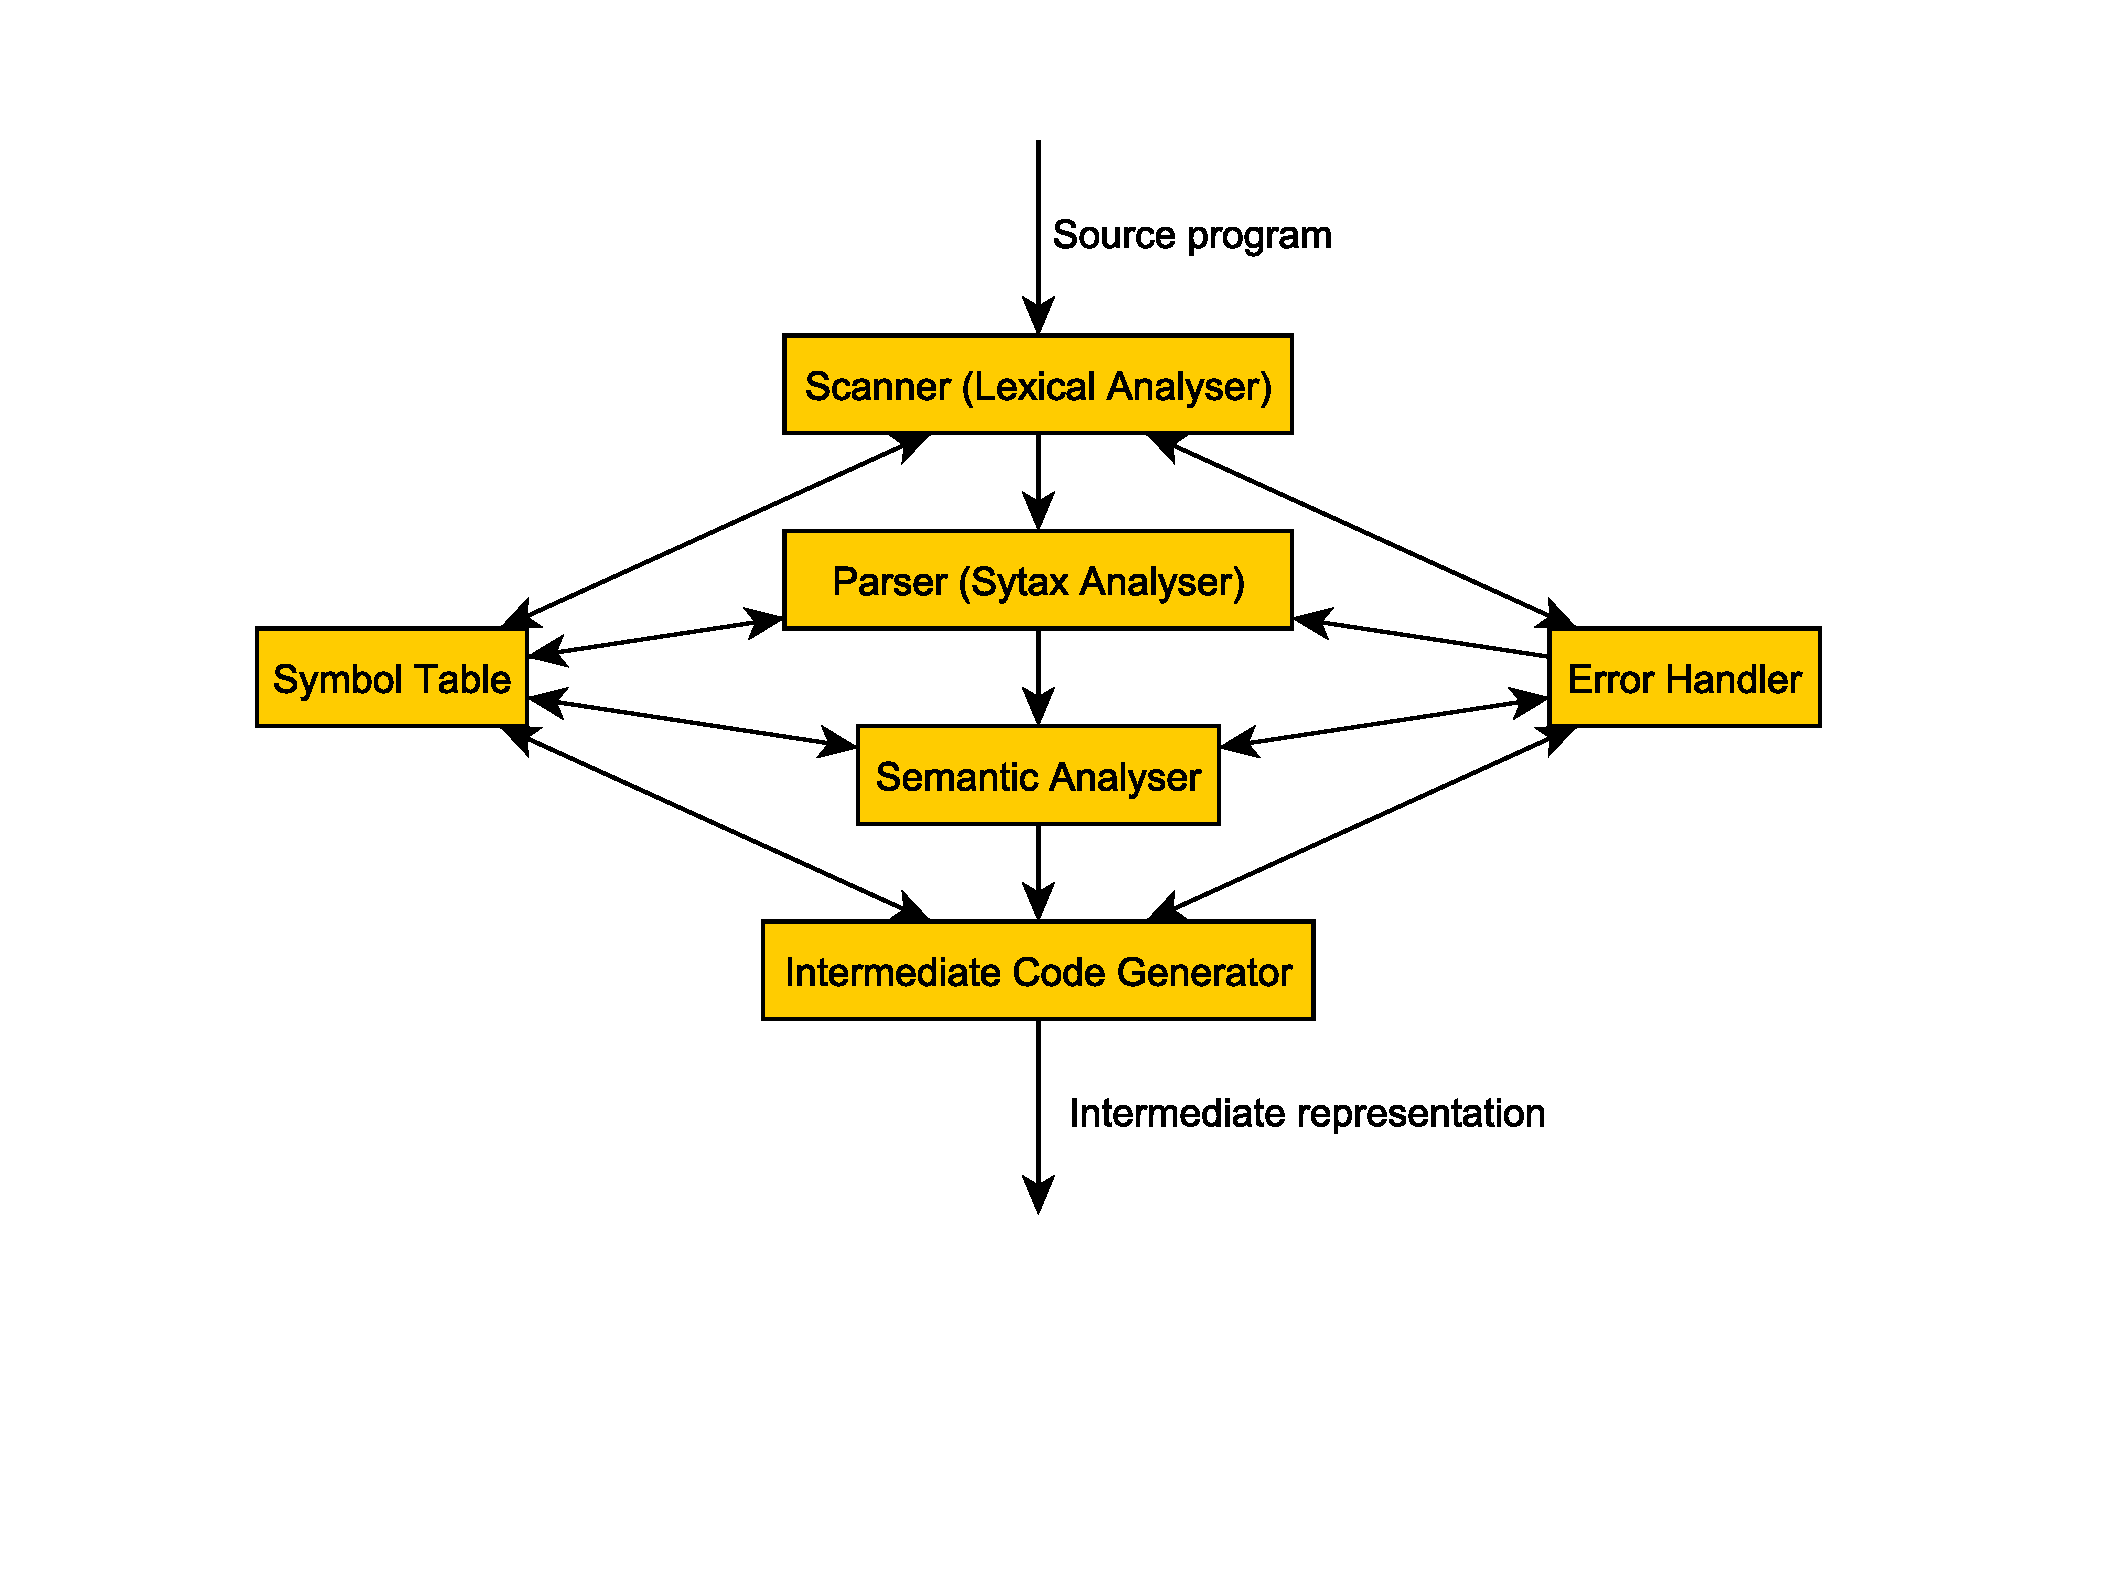
\includegraphics[width=0.8\textwidth]{img/11.pdf}}
\end{figure}

\subsection{Back-End}
\begin{figure}[H]
    \centerline{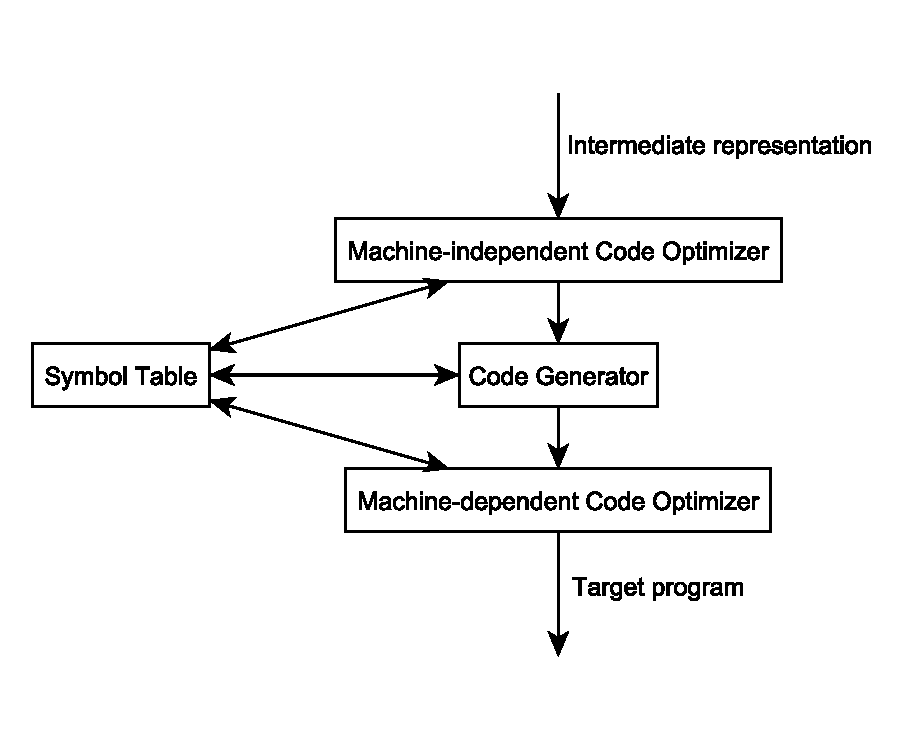
\includegraphics[width=0.8\textwidth]{img/12.pdf}}
\end{figure}

\chapter{Lexical Analysis (LA)}

\chapter{Syntax Analysis (SA)}

\chapter{Syntax-Directed Translation (SDT)}

\chapter{Semantic Analysis and Intermediate-Code Generation (SA/ICG)}

\end{document}
